%
% assembly.tex
%
% Copyright (C) 2021 by SpaceLab.
%
% TTC Documentation
%
% This work is licensed under the Creative Commons Attribution-ShareAlike 4.0
% International License. To view a copy of this license,
% visit http://creativecommons.org/licenses/by-sa/4.0/.
%

%
% \brief Assembly instructions chapter.
%
% \author Gabriel Mariano Marcelino <gabriel.mm8@gmail.com>
%
% \institution Universidade Federal de Santa Catarina (UFSC)
%
% \version 1.2.0
%
% \date 2021/01/16
%

\chapter{Assembly Instructions} \label{ch:assembly}

\section{Radio Configuration}

This appendix is a tutorial with the purpose of generate a source code file with basic configuration parameters of the radio module. For it, the WDS software from Silicon Labs will be used (version 3.2.11.0).

Unfortunately, the software in only available for Windows platforms.

\subsection{Steps}

After the installation of the software, the procedures to configure the beacon radio are described bellow (When a parameter to configure the telemetry link radio differs from the beacon radio, a note describes the difference).

\subsubsection{Step 1}

\begin{enumerate}
    \item Open the WDS software.
    \item The following box will appear in the center of the window.
    \item Click in "Simulate radio" and go to the next step.
\end{enumerate}

\begin{figure}[!h]
	\begin{center}
		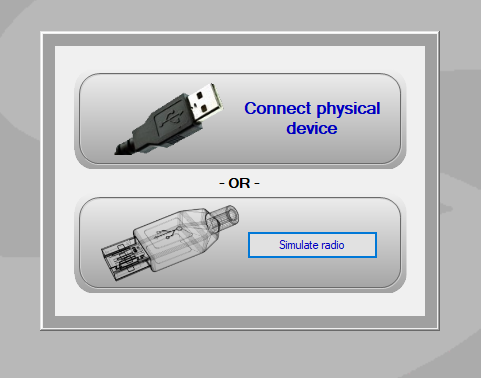
\includegraphics[width=0.5\textwidth]{figures/wds-tutorial-1.png}
		\caption{Step 1 of the radio configuration.}
		\label{fig:wds-tutorial-step-1}
	\end{center}
\end{figure}

\subsubsection{Step 2}

\begin{enumerate}
    \item In the list of radios that appeared on the new window, select the chip type ``Si4463".
    \item In the revision column, select ``B1".
    \item Click on ``Select Radio" to go to the next step.
\end{enumerate}

\begin{figure}[!h]
	\begin{center}
		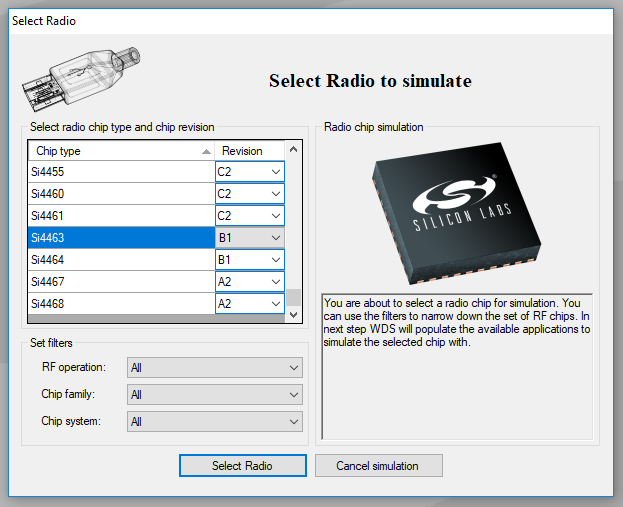
\includegraphics[width=0.75\textwidth]{figures/wds-tutorial-2.png}
		\caption{Step 2 of the radio configuration.}
		\label{fig:wds-tutorial-step-2}
	\end{center}
\end{figure}

\subsubsection{Step 3}

\begin{enumerate}
    \item Select ``Radio Configuration Application".
    \item Click on ``Select Application" to go to the next step.
\end{enumerate}

\begin{figure}[!h]
	\begin{center}
		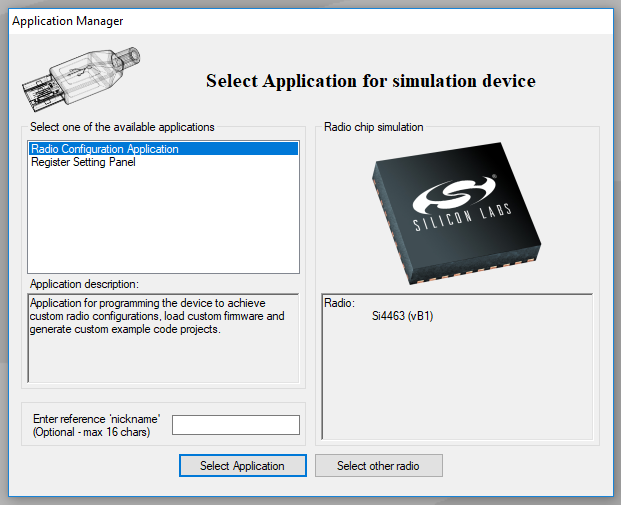
\includegraphics[width=0.75\textwidth]{figures/wds-tutorial-3.png}
		\caption{Step 3 of the radio configuration.}
		\label{fig:wds-tutorial-step-3}
	\end{center}
\end{figure}

\subsubsection{Step 4}

\begin{enumerate}
    \item In the ``Frequency and power" tab, change the base frequency to 145,9 MHz.
    \item Change the channel spacing to 0 kHz.
    \item Change the crystal tolerance to 10,0 ppm (Both RX and TX).
    \item Go to the next step.
\end{enumerate}

\begin{figure}[!h]
	\begin{center}
		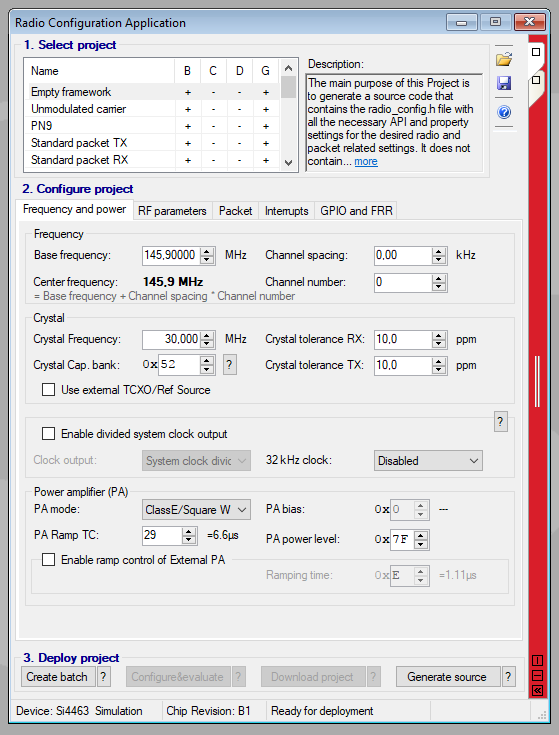
\includegraphics[width=0.75\textwidth]{figures/wds-tutorial-4.png}
		\caption{Step 4 of the radio configuration.}
		\label{fig:wds-tutorial-step-4}
	\end{center}
\end{figure}

\subsubsection{Step 5}

\begin{enumerate}
    \item In the ``RF parameters" tab, change the modulation type to ``2GFSK".
    \item Change the the data rate to 1,2 kbps.
    \item Change the deviation to $2,5\ kHz$.
    \item Go to the next step.
\end{enumerate}

\begin{figure}[!h]
	\begin{center}
		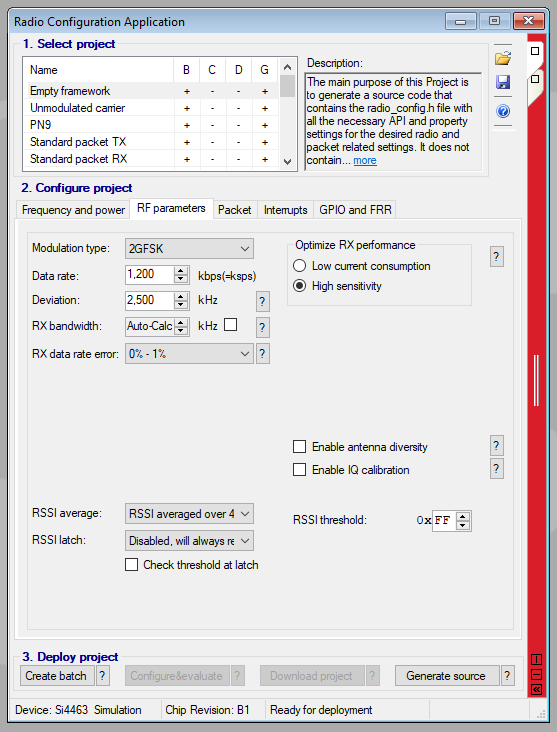
\includegraphics[width=0.75\textwidth]{figures/wds-tutorial-5.png}
		\caption{Step 5 of the radio configuration.}
		\label{fig:wds-tutorial-step-5}
	\end{center}
\end{figure}

\subsubsection{Step 6}

\begin{enumerate}
    \item In the ``Packet" tab, many subtabs will appear. In ``Preamble" change the ``Preamble TX length" to 4 bytes.
    \item Again, in ``Preamble", change the ``Preamble pattern" to ``Std. 1010 pattern (>= 32 and < 40 bits)".
    \item Go to the next step.
\end{enumerate}

\begin{figure}[!h]
	\begin{center}
		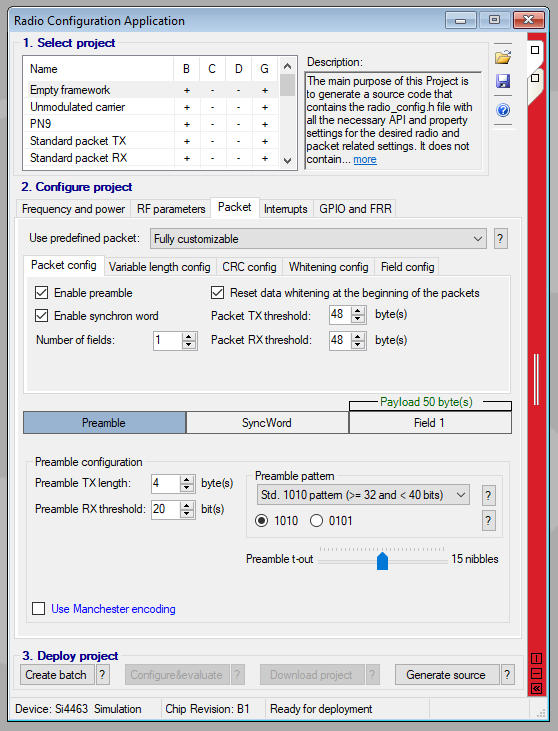
\includegraphics[width=0.75\textwidth]{figures/wds-tutorial-6.png}
		\caption{Step 6 of the radio configuration.}
		\label{fig:wds-tutorial-step-6}
	\end{center}
\end{figure}

\subsubsection{Step 7}

\begin{enumerate}
    \item In the ``Sync Word" tab, change the sync word length field to ``4 bytes".
    \item In the ``Sync Word (on air int.)", enter the following sequence: 5D E6 2A 7E. This sequence is the sync word used by the NGHam protocol.
    \item Go to the next step.
\end{enumerate}

\begin{figure}[!h]
	\begin{center}
		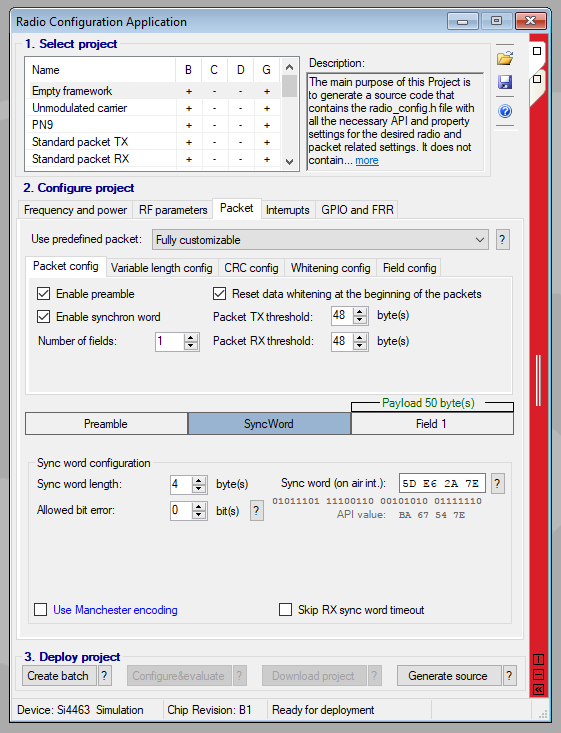
\includegraphics[width=0.75\textwidth]{figures/wds-tutorial-7.png}
		\caption{Step 7 of the radio configuration.}
		\label{fig:wds-tutorial-step-7}
	\end{center}
\end{figure}

\subsubsection{Step 8}

\begin{enumerate}
    \item In the ``Field 1" tab, change the ``Field length" to 50 bytes.
    \item Go to the next step.
\end{enumerate}

\begin{figure}[!h]
	\begin{center}
		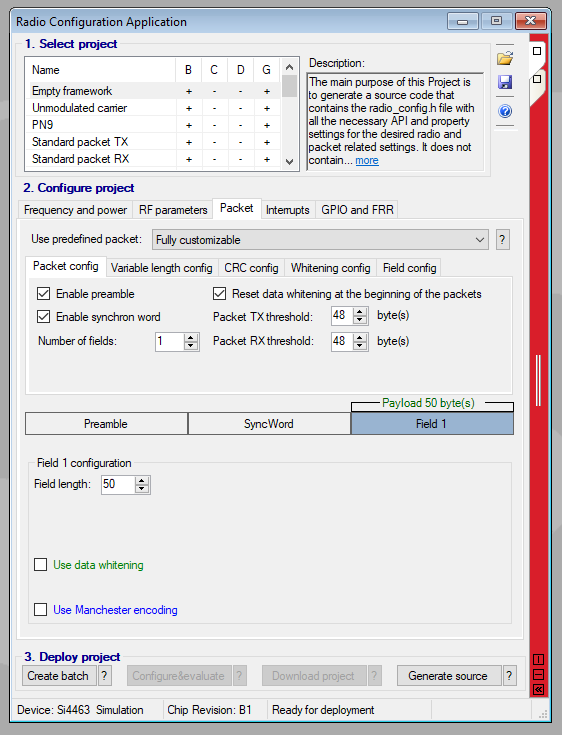
\includegraphics[width=0.75\textwidth]{figures/wds-tutorial-8.png}
		\caption{Step 8 of the radio configuration.}
		\label{fig:wds-tutorial-step-8}
	\end{center}
\end{figure}

\subsubsection{Step 9}

\begin{enumerate}
    \item In the ``Variable length config" tab, there is no values to change.
    \item Go to the next step.
\end{enumerate}

\begin{figure}[!h]
	\begin{center}
		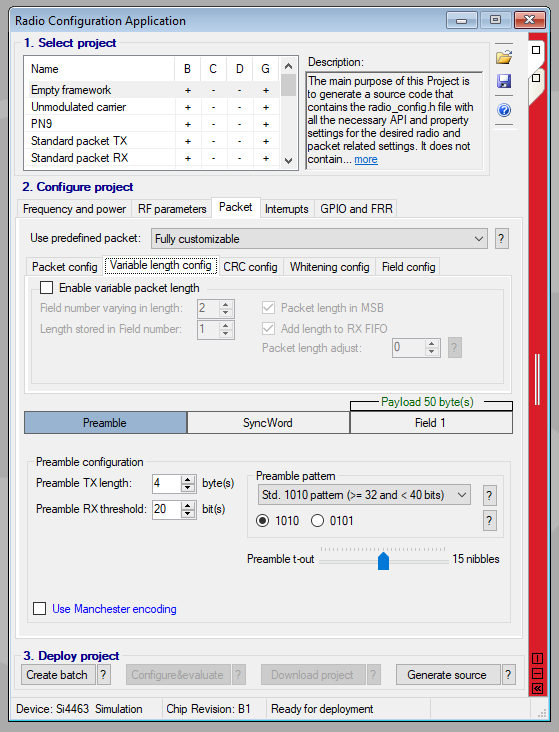
\includegraphics[width=0.75\textwidth]{figures/wds-tutorial-9.png}
		\caption{Step 9 of the radio configuration.}
		\label{fig:wds-tutorial-step-9}
	\end{center}
\end{figure}

\subsubsection{Step 10}

\begin{enumerate}
    \item In the ``CRC config" tab, choose ``No CRC." in ``CRC polynomial".
    \item Go to the next step.
\end{enumerate}

\begin{figure}[!h]
	\begin{center}
		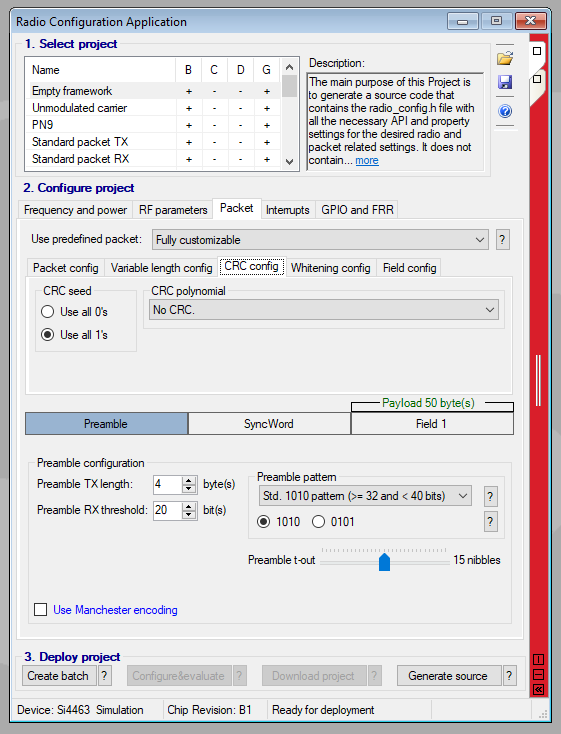
\includegraphics[width=0.75\textwidth]{figures/wds-tutorial-10.png}
		\caption{Step 10 of the radio configuration.}
		\label{fig:wds-tutorial-step-10}
	\end{center}
\end{figure}

\subsubsection{Step 11}

\begin{enumerate}
    \item In the ``Whitening config" tab, there is no values to change.
    \item Go to the next step.
\end{enumerate}

\begin{figure}[!h]
	\begin{center}
		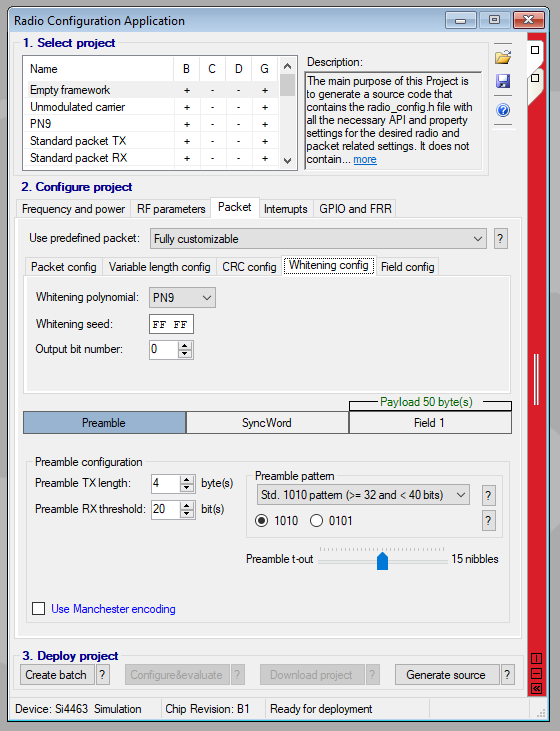
\includegraphics[width=0.75\textwidth]{figures/wds-tutorial-11.png}
		\caption{Step 11 of the radio configuration.}
		\label{fig:wds-tutorial-step-11}
	\end{center}
\end{figure}

\subsubsection{Step 12}

\begin{enumerate}
    \item In the ``Field config" tab, there is no values to change.
    \item Go to the next step.
\end{enumerate}

\begin{figure}[!h]
	\begin{center}
		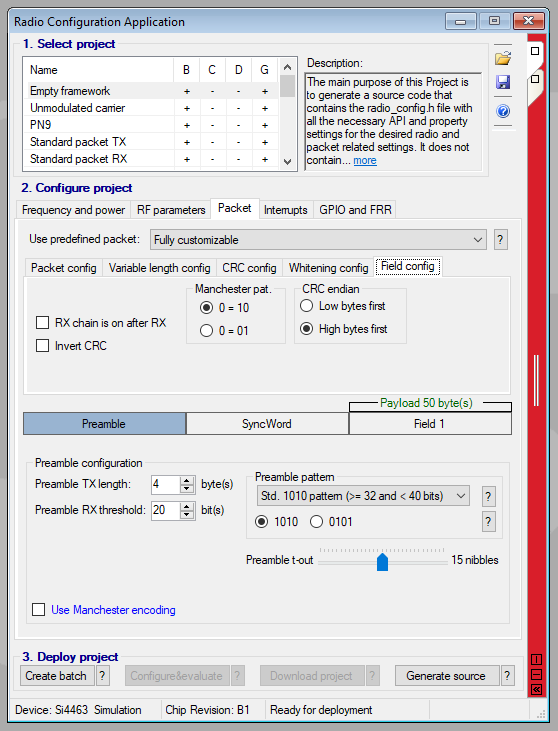
\includegraphics[width=0.75\textwidth]{figures/wds-tutorial-12.png}
		\caption{Step 12 of the radio configuration.}
		\label{fig:wds-tutorial-step-12}
	\end{center}
\end{figure}

\subsubsection{Step 13}

\begin{enumerate}
    \item In the ``Interrupts" tab, there is no values to change.
    \item Go to the next step.
\end{enumerate}

\begin{figure}[!h]
	\begin{center}
		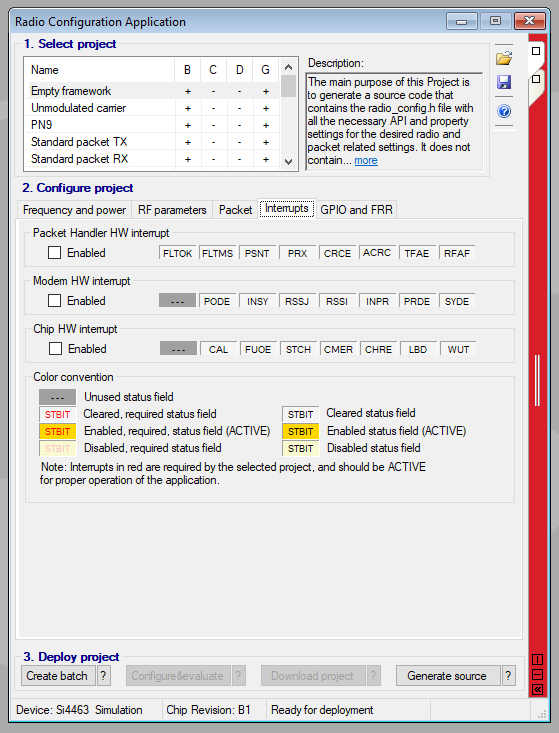
\includegraphics[width=0.75\textwidth]{figures/wds-tutorial-13.png}
		\caption{Step 13 of the radio configuration.}
		\label{fig:wds-tutorial-step-13}
	\end{center}
\end{figure}

\subsubsection{Step 14}

\begin{enumerate}
    \item In the ``GPIO and FRR" tab, enable pullup in GPIO1 and choose ``TX\_FIFO\_EMPTY - This output is..." as functionality.
    \item Enable pullup in GPIO2 and choose ``RX\_STATE - This output is..." as functionality.
    \item Enable pullup in GPIO3 and choose ``TX\_STATE - This output is..." as functionality.
    \item Enable pullup in NIRQ and choose ``Active low interrupt signal" as functionality.
    \item Enable pullup in SDO and choose ``SDO - Output SPI Serial data out." as functionality.
    \item Select ``Global status" for the ``Fast Response Register A".
    \item Select ``Global interrupt status" for the ``Fast Response Register B".
    \item Select ``Packet Handler status" for the ``Fast Response Register C".
    \item Select ``Chip status status" for the ``Fast Response Register D".
    \item Go to the next step.
\end{enumerate}

\begin{figure}[!h]
	\begin{center}
		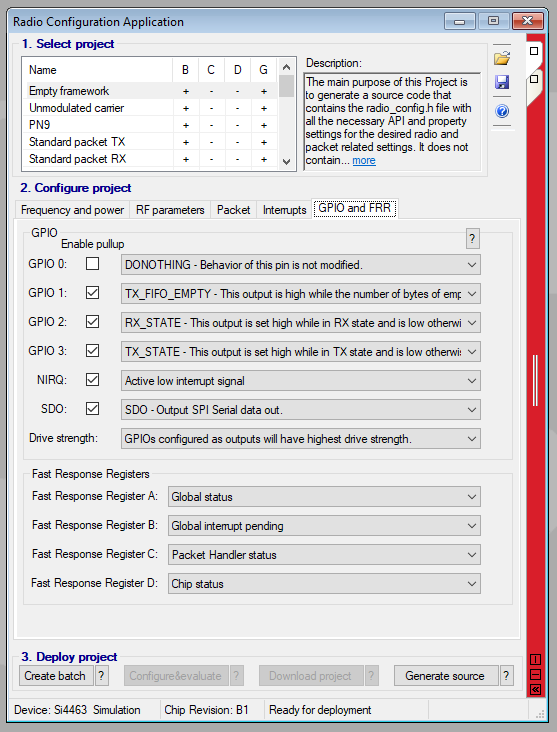
\includegraphics[width=0.75\textwidth]{figures/wds-tutorial-14.png}
		\caption{Step 14 of the radio configuration.}
		\label{fig:wds-tutorial-step-14}
	\end{center}
\end{figure}

\subsubsection{Step 15}

\begin{enumerate}
    \item Click in ``Generate Source" and select the ``.h" type of source.
    \item The software will ask where to save the generated file.
    \item The generated *.h file must be copied to the directory of the rf4463 driver.
\end{enumerate}

\subsection{Final Remarks}

This tutorial has the objective of generate a basic configuration parameters of the radio, some functionalities of the radio are not covered by the WDS software, and so, must be configured/controlled in the device driver.

\section{Compiling and Building the Beacon Firmware}

This tutorial is a reference to compile, build and flash the firmware of the beacon of the TTC module. All the software development was made using the Code Composer Studio (CCS) IDE, version 7.3.0. To load the code into the TTC MCU, the MSP-FET can be used.

\subsection{Creating the Project}

After the download and installation of the CCS, open it and create a new project with following steps:

\begin{enumerate}
    \item Go to ``File" -> ``New" -> ``CCS Project".
    \item The window from the figure \ref{fig:compiling-tutorial} will appear on the screen.
    \item On ``Target", select MSP430F6659.
    \item On ``Project name", enter the name of the project (It can be ``beacon", ``beacon\_firmware", or whatever name you want).
    \item On ``Project templates and examples" box, select ``Empty project".
    \item Click on ``Finish".
\end{enumerate}

\begin{figure}[!h]
	\begin{center}
		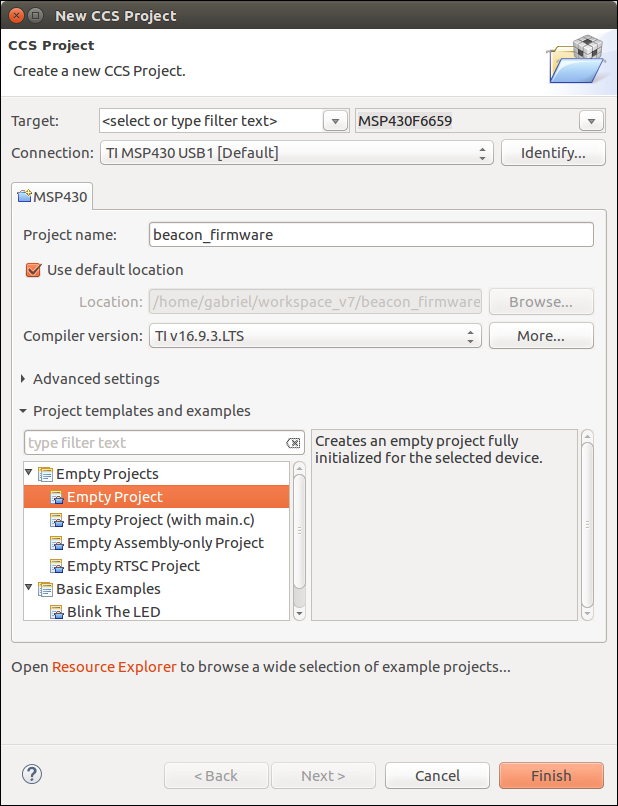
\includegraphics[width=0.75\textwidth]{figures/ccs_project.png}
		\caption{New CCS project window.}
		\label{fig:compiling-tutorial}
	\end{center}
\end{figure}

Now the beacon project with the correct parameters has been created, and the project source code files must be moved to the project directory. Copy the files inside the ``beacon" folder from the TTC git repository to the project folder.

\subsection{Compiling and Building}

To compile and build the firmware, click on "Project" -> "Build Project". If the process finish with no errors, the code is ready to go to the MCU of the beacon.

\subsection{Flashing}

To load the code into the board, connect the MSP-FET in the computer and follow the power-on tutorial.

With the board turned on and the MSP-FET connected, click on ``Run" -> ``Debug" or just press F11. If no errors occur, the firmware was loaded succesfully to the board.

\section{Power-On the TTC Module}

To power-on the TTC module, there are three different possibilities:

\begin{enumerate}
    \item Using three different power sources: one for the MCU, one for the beacon radio module and one for the telemetry radio module.
    \item Using two different power sources: one for each radio module (in this case, the beacon MCU is powered using the JTAG bus).
    \item Using just one power source to all components (THIS METHOD IS NOT SAFE: there is no control over the power consumption of each component).
\end{enumerate}

To test just the beacon, there is no need to power-on the telemetry radio module. Turning on the telemetry radio only makes sense if an external module is connected and controlling it (Like an OBC or an OBDH).

The connections reference of the TTC board can be found in External Connections.

\subsection{Using an External Power Source for the Beacon MCU}

\subsubsection{Power-On the Beacon MCU}

\begin{enumerate}
    \item Set an output of a channel of the power source to $3,3\ V$ and $30\ mA$ (Cut-off current).
    \item Connect the positive cable to the H2A-14 or H2B-14 pin of the PCI-104 connector.
    \item Connect the ground cable to any GND pin of the PCI-104 connector.
    \item Turn on this channel of the power source.
\end{enumerate}

\subsubsection{Power-On the Beacon Radio Module}

\begin{enumerate}
    \item Set another output of a channel of the power source to $5,0\ V$ and $500\ mA$ (Cut-off current).
    \item Connect the positive cable to the H1A-26 pin of the PCI-104 connector.
    \item Connect the ground cable to any GND pin of the PCI-104 connector.
    \item Turn on this channel of the power source.
\end{enumerate}

\subsubsection{Power-On the Telemetry Radio Module}

\begin{enumerate}
    \item Set another output of a channel of the power source to $5,0\ V$ and $500\ mA$ (Cut-off current).
    \item Connect the positive cable to the H1A-25 pin of the PCI-104 connector.
    \item Connect the ground cable to any GND pin of the PCI-104 connector.
    \item Turn on this channel of the power source.
\end{enumerate}

\subsection{Using the JTAG as Power Source for the Beacon MCU}

In this case, to power on the beacon MCU, just connect a jumper in the P4 connector of the board and after, connect a MSP-FET debbuger to the JTAG connector.

The procedure to power-on the radio modules is the same as above.

\section{Receiving the Beacon Data}

\subsection{Required Softwares}

\begin{itemize}
    \item GQRX (For just receive the signal).
    \item RTL-SDR drivers (The GRQX will install all the required drivers).
    \item FloripaSat GRS (For receive the signal and data).
\end{itemize}

\subsubsection{Supported SDRs}

\begin{itemize}
    \item RTL-SDR
    \item FunCube Dongle Pro+
\end{itemize}

\subsection{Receiving the Beacon Signal}

In this method, you will not be able to see the beacon data in real time. This only shows the presence of the beacon signals in the air.

The instructions to receive the beacon signal in the GQRX are available bellow:

\begin{enumerate}
    \item Open the GQRX software.
    \item Configure it for your SDR model.
    \item Press the power button on the upper left corner.
    \item Select the frequency to 145,9 MHz.
    \item Wait the spectrum of the beacon signal appear.
\end{enumerate}

The figure \ref{fig:beacon-signal-gqrx} illustrates the reception of the beacon signal in the GQRX software.

\begin{figure}[!h]
	\begin{center}
		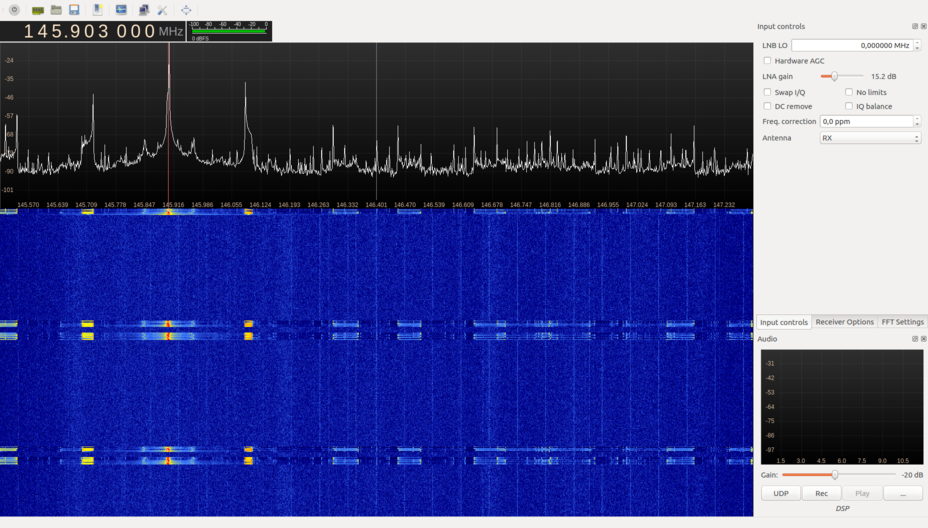
\includegraphics[width=\textwidth]{figures/beacon-signal-gqrx.png}
		\caption{Beacon signal in GQRX.}
		\label{fig:beacon-signal-gqrx}
	\end{center}
\end{figure}

\subsection{Receiving the Beacon Data}

Using this method, you will be able to see the beacon (and the telemetry) data in real time on the computer screen. For that, the FloripaSat GRS sofware is required.

\begin{enumerate}
    \item Open the FloripaSat GRS software.
    \item Connect a the SDR device.
    \item Select the source of the signal.
    \item Press the play button in the beacon frame.
    \item A new window will appear in the screen, with the FFT and Waterfall plot of the received signal (in real time) of the connected SDR.
    \item Power on the beacon module of the TTC board.
    \item Adjust the frequency of the receive to the center frequency of the beacon signal (Use the FFT and the Waterfall plot for that).
    \item With the correct frequency sinthonization, the beacon data should appear in the main window of the FloripaSat GRS softwate.
\end{enumerate}

\begin{figure}[!h]
	\begin{center}
		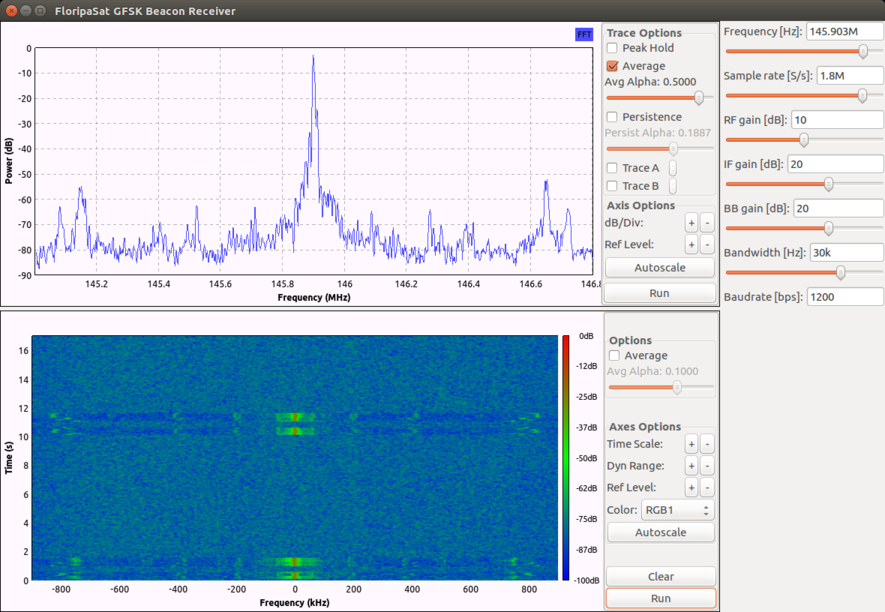
\includegraphics[width=\textwidth]{figures/beacon-signal-gnuradio.png}
		\caption{Beacon signal in the GNURadio receiver from the FloripaSat GRS.}
		\label{fig:beacon-signal-gnuradio}
	\end{center}
\end{figure}

\begin{figure}[!h]
	\begin{center}
		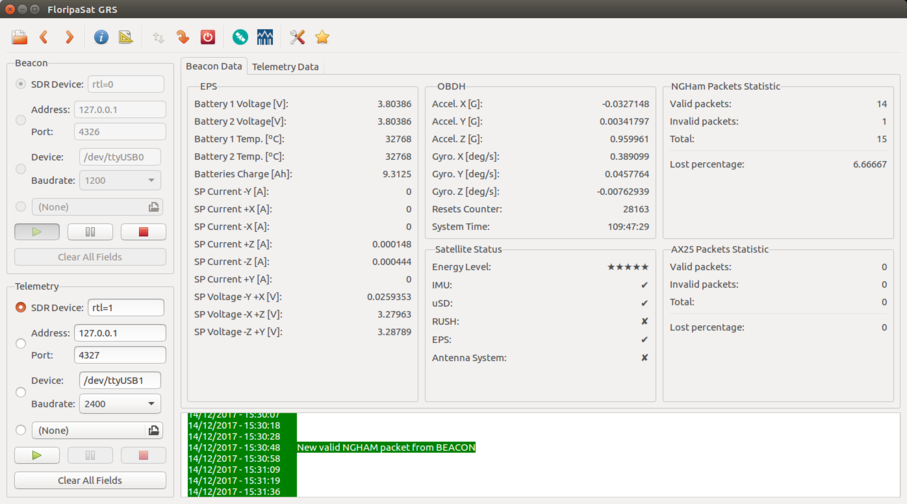
\includegraphics[width=\textwidth]{figures/beacon-data-grs.png}
		\caption{Beacon data in the FloripaSat GRS.}
		\label{fig:beacon-data-grs}
	\end{center}
\end{figure}
